\subsection{Theory Crafting Next steps}

For the remaining duration, we will focus on three main objectives:
One will be to demonstrate that, the \textit{bipolar} colouring
of \textsc{nD-StrongSperner} will keep the reduction parsimonious.
Second, will be to demonstrate hardness over \textsc{\#P} class either by finding
reductions from the \textsc{SourceOrExcess} problem.
And lastly, we will be to generalise our reduction to all $\#PPAD$ problems.


\subsection{Software Next Steps}

In the next steps we aim to complete the rest of the milestones. 
We believe that the usage of methods by Eichelberger et al. \cite{eichelberger_HazardDetectionCombinational_1965}
and or polynomial algorithm for specific cases by \cite{deligkas_PureCircuitTightInapproximability_2024}
will allow us to identify solutions. With regards to counting, we can only hope
to count solutions for small instances.


\subsection{Timetable}

The figure \ref{fig:gantt-new} depicts how the remaining project will progress with regards
to the milestones we aim to achieve. Overall we modified our timeline to prioritise
theory crafting and therefore we hope this adjusted timeline will capture accurately the remaining duration
of the project.

\begin{figure}[h!]
    \centering
    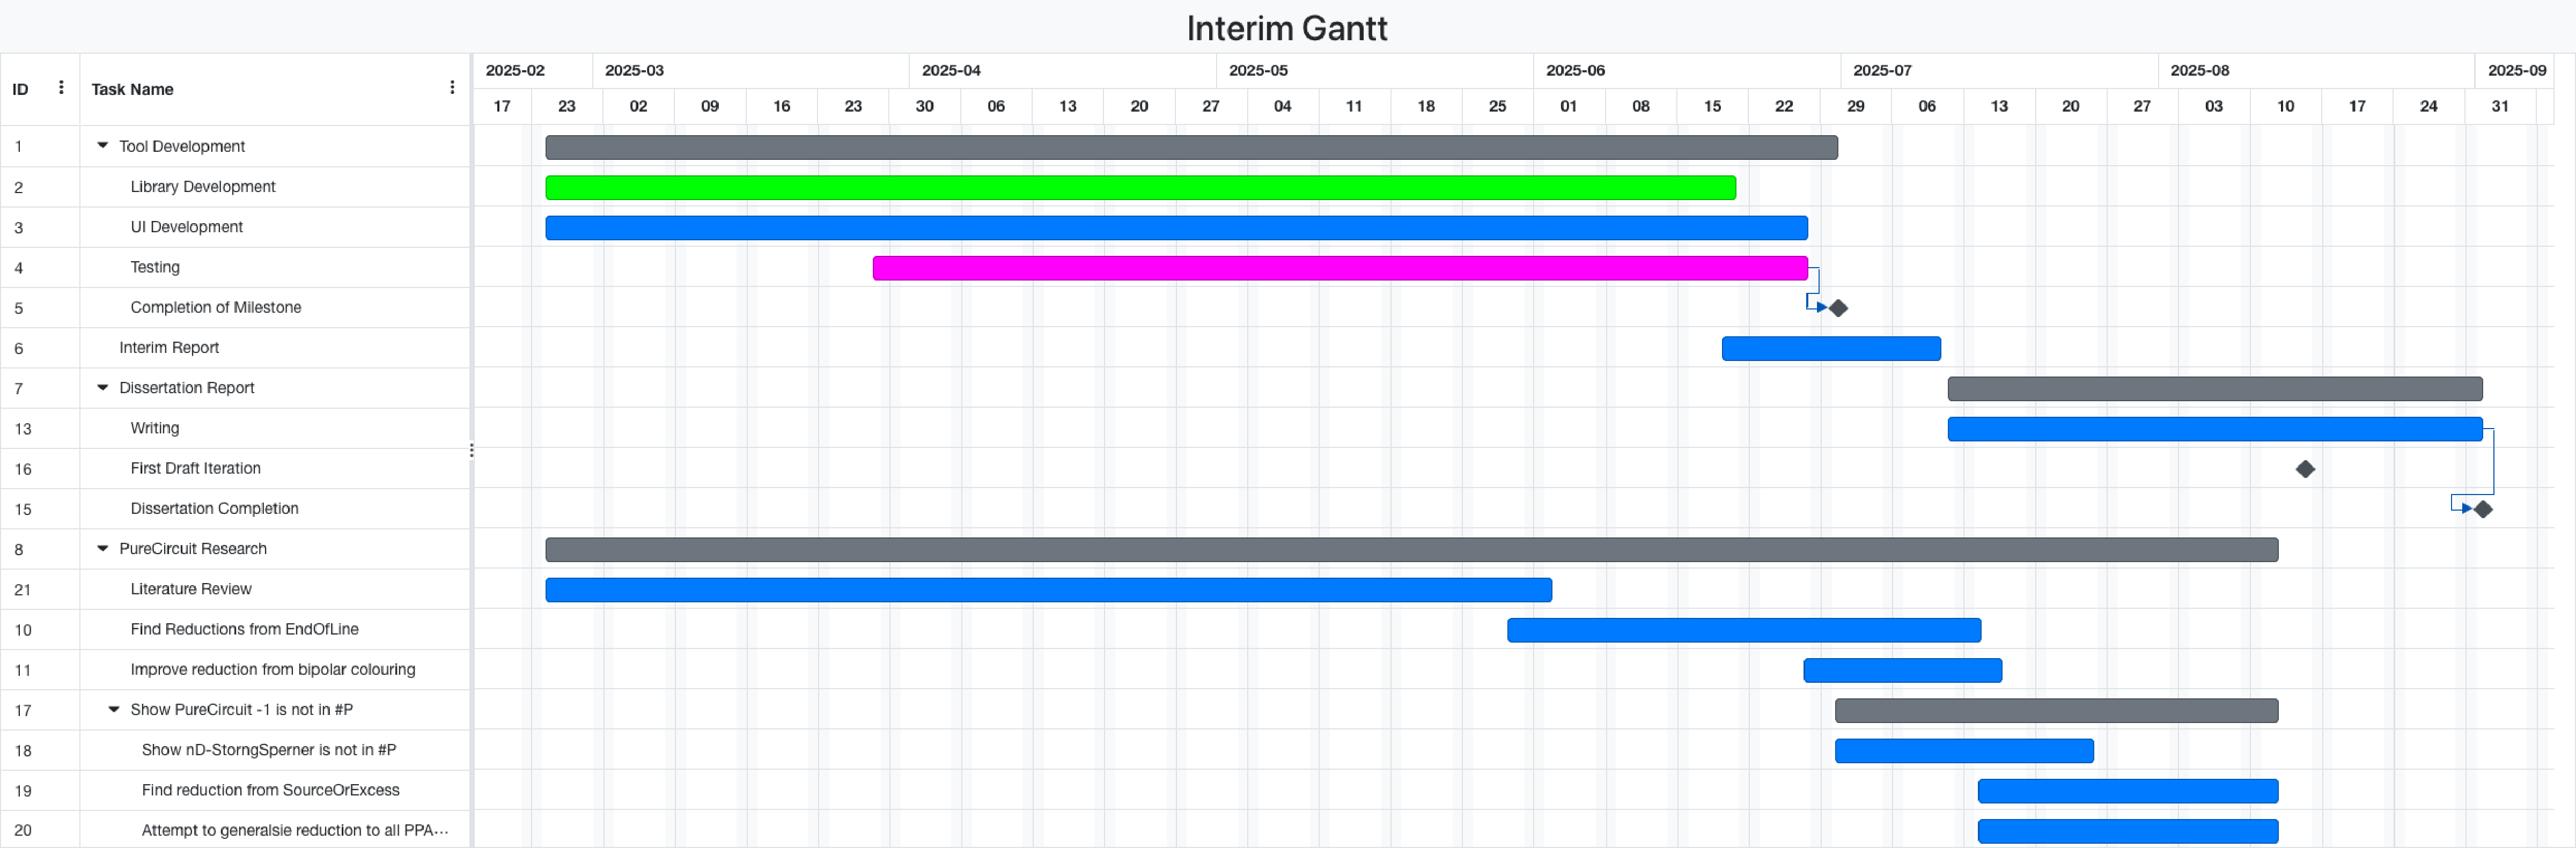
\includegraphics[width=0.85\textwidth]{assets/Interim Gantt 20250708.pdf}
    \caption{Updated Gantt chart}\label{fig:gantt-new}
\end{figure}

